\documentclass[a4paper,11pt]{article}

\usepackage[utf8]{inputenc}
\usepackage{polski}
\usepackage{hyperref}
\usepackage[vmargin=0.7in, hmargin=0.9in]{geometry}
\usepackage{graphicx}
\usepackage{subcaption}
\usepackage{listings}
\usepackage{xcolor}
\definecolor{backcolour}{rgb}{.9, .9, .9}
\lstset{backgroundcolor=\color{backcolour}, basicstyle=\ttfamily\scriptsize, breaklines=true}

\title{Zaawansowane Bazy Danych 2020\\
\large zadanie 2}

\author{Kamil Dubil\\
\href{mailto:kd370826@students.mimuw.edu.pl}{\tt kd370826@students.mimuw.edu.pl}}


\begin{document}

\maketitle

Dane, skrypty i wykresy generuję w Rubym.


\section{Generator danych}

Domyślną liczbą dni jest 60, liczbą kategorii i kolumn z wartościami --- 10.
W celu przetestowania wydajności w zależności od tych parametrów, generuję dane ze zmienionymi pojedynczymi wartościami.
Dla \texttt{number\_of\_days} dni, \texttt{number\_of\_categories} kategorii i \texttt{number\_of\_values} kolumn z~wartościami,
dane mają $2 + \texttt{number\_of\_values}$ kolumn i \texttt{number\_of\_days} $\cdot$ \texttt{number\_of\_categories} wierszy.

\begin{lstlisting}
require 'date'
require 'csv'
require 'distribution'

START_DATE = Date.new(2020, 1, 1)
DATES = (START_DATE..).first(10_000)
CATEGORIES = ('A'..).first(1000)
VALUES = ('value_1'..).first(1000)
MEAN = 0
STANDARD_DEVIATION = 10

def generate_data(number_of_days: 60, number_of_categories: 10, number_of_values: 10)
  normal = Distribution::Normal.rng(MEAN, STANDARD_DEVIATION)
  CSV.open("./data/data-#{number_of_days}-#{number_of_categories}-#{number_of_values}.csv", 'wb') do |csv|
    DATES.first(number_of_days).each do |date|
      number_of_categories.times do |c|
        row = [date, CATEGORIES[c]]
        row += number_of_values.times.map{ normal.call.to_i }
        csv << row
      end
    end
  end
end

NUMBERS_OF_VALUES_AND_CATEGORIES = [1, 50, 100, 150, 200, 250, 300, 350, 400, 450, 500, 550, 600, 650, 700, 750, 800]
DISTANCES_IN_DAYS = [1, 100, 200, 300, 400, 500, 1000, 2000, 3000, 4000, 5000, 6000, 7000]

NUMBERS_OF_VALUES_AND_CATEGORIES.each do |n|
  generate_data(number_of_values: n)
  generate_data(number_of_categories: n)
end

generate_data(number_of_days: 8000)
\end{lstlisting}


\section{Zapytania}

W każdej z trzech wersji zapytania są identyczne, postaci:
\begin{lstlisting}
-- query1: suma wartosci k w przedziale dat date_from, date_to
SELECT SUM(value_k)
FROM data
WHERE date BETWEEN date_from AND date_to;
-- query2: suma wartosci k kategorii j w przedziale dat date_from, date_to
SELECT SUM(value_k)
FROM data
WHERE date BETWEEN date_from AND date_to AND category = j;
\end{lstlisting}
Generuję je w następujący sposób:
\begin{lstlisting}
def explain_analyze_queries(name, key, number_of_days, number_of_categories, number_of_values, table_name)
  if name == 'distance_in_days'
    date_from = DATES.first(number_of_days - key).sample
    date_to = date_from + key
  else
    date_from, date_to = DATES.first(number_of_days).sample(2).sort
  end
  value = VALUES.first(number_of_values).sample

  %{
ANALYZE #{table_name};

\\echo 'Execution Time: #{name} query1 #{key}'

EXPLAIN ANALYZE
SELECT SUM(#{value})
FROM #{table_name}
WHERE date BETWEEN '#{date_from.to_s}' AND '#{date_to.to_s}';

\\echo 'Execution Time: #{name} query2 #{key}'

EXPLAIN ANALYZE
SELECT SUM(#{value})
FROM #{table_name}
WHERE date BETWEEN '#{date_from.to_s}' AND '#{date_to.to_s}' AND category = '#{CATEGORIES.first(number_of_categories).sample}';
}
end
\end{lstlisting}

Dodatkowo generuję zapytania do przetestowania rozmiaru plików z danymi:
\begin{lstlisting}
def size_of_data_file(name, key, table_name)
  %{
\\echo 'Size of data file: #{name} #{key}'

SELECT 'Size of data file: ' || #{table_name == 'cstore_data' ? "cstore_table_size('cstore_data')" : "(pg_stat_file(pg_relation_filepath('#{table_name}'))).size"};
}
end
\end{lstlisting}


\subsection{Wersja korzystająca z \texttt{file\_fdw}}

Na początku, jednorazowo:
\begin{lstlisting}
DROP EXTENSION IF EXISTS file_fdw;
CREATE EXTENSION file_fdw;

DROP SERVER IF EXISTS csv_data_server;
CREATE SERVER csv_data_server FOREIGN DATA WRAPPER file_fdw;
\end{lstlisting}
Potem zapytania dla tej wersji generuję za pomocą metody:
\begin{lstlisting}
def generate_file_fdw_script(name:, key:, number_of_days: 60, number_of_categories: 10, number_of_values: 10)
  %{
DROP FOREIGN TABLE IF EXISTS csv_data;
CREATE FOREIGN TABLE csv_data (
    date date NOT NULL,
    category text NOT NULL,
    #{VALUES.first(number_of_values).map{ |v| "#{v} int NOT NULL" }.join(",\n    ")}
)
SERVER csv_data_server
OPTIONS (
    filename '/home/kd/zbd/zad2/data/data-#{number_of_days}-#{number_of_categories}-#{number_of_values}.csv',
    format 'csv'
);

#{explain_analyze_queries(name, key, number_of_days, number_of_categories, number_of_values, 'csv_data')}

DROP FOREIGN TABLE IF EXISTS csv_data;
}
end
\end{lstlisting}


\subsection{Wersja korzystająca z jednej tabeli w postgresie}

Zapytania generuję metodą:
\begin{lstlisting}
def generate_sql_one_table_script(name:, key:, number_of_days: 60, number_of_categories: 10, number_of_values: 10, primary_key: true)
  %{
DROP TABLE IF EXISTS csv_data;
CREATE TABLE csv_data (
    date date NOT NULL,
    category text NOT NULL,
    #{'PRIMARY KEY (date, category),' if primary_key}
    #{VALUES.first(number_of_values).map{ |v| "#{v} int NOT NULL" }.join(",\n    ")}
);

COPY csv_data FROM '/home/kd/zbd/zad2/data/data-#{number_of_days}-#{number_of_categories}-#{number_of_values}.csv' (FORMAT 'csv');

#{size_of_data_file(name, key, 'csv_data')}

#{explain_analyze_queries(name, key, number_of_days, number_of_categories, number_of_values, 'csv_data')}

DROP TABLE IF EXISTS csv_data;
}
end
\end{lstlisting}


\subsection{Wersja korzystająca z \texttt{cstore\_fdw}}

Na początku, po zbudowaniu i dodaniu w pliku konfiguracyjnym rozszerzenia, jednorazowo:
\begin{lstlisting}
DROP EXTENSION IF EXISTS cstore_fdw;
CREATE EXTENSION cstore_fdw;

DROP SERVER IF EXISTS cstore_server;
CREATE SERVER cstore_server FOREIGN DATA WRAPPER cstore_fdw;
\end{lstlisting}
Potem zapytania generuję za pomocą metody:
\begin{lstlisting}
def generate_cstore_fdw_script(name:, key:, number_of_days: 60, number_of_categories: 10, number_of_values: 10)
  %{
DROP FOREIGN TABLE IF EXISTS cstore_data;
CREATE FOREIGN TABLE cstore_data (
    date date NOT NULL,
    category text NOT NULL,
    #{VALUES.first(number_of_values).map{ |v| "#{v} int NOT NULL" }.join(",\n    ")}
)
SERVER cstore_server;

COPY cstore_data FROM '/home/kd/zbd/zad2/data/data-#{number_of_days}-#{number_of_categories}-#{number_of_values}.csv' (FORMAT 'csv');

#{size_of_data_file(name, key, 'cstore_data')}

#{explain_analyze_queries(name, key, number_of_days, number_of_categories, number_of_values, 'cstore_data')}

DROP FOREIGN TABLE IF EXISTS cstore_data;
}
end
\end{lstlisting}


\subsection{Ostateczne zapytania}

Dla każdej wersji generuję 10 skryptów (różniących się z powodu losowego wyboru dat, kategorii i~sumowanych wartości),
aby później obliczyć średnią otrzymanych czasów wykonania.
\begin{lstlisting}
10.times do |i|
  File.open("./scripts/file-fdw-full-#{i}.sql", 'w') do |file|
    NUMBERS_OF_VALUES_AND_CATEGORIES.each do |n|
      file.write generate_file_fdw_script(name: 'number_of_values', key: n, number_of_values: n)
      file.write generate_file_fdw_script(name: 'number_of_categories', key: n, number_of_categories: n)
    end

    DISTANCES_IN_DAYS.each do |n|
      file.write generate_file_fdw_script(name: 'distance_in_days', key: n, number_of_days: 8000)
    end
  end

  File.open("./scripts/sql-one-table-full-#{i}.sql", 'w') do |file|
    NUMBERS_OF_VALUES_AND_CATEGORIES.each do |n|
      file.write generate_sql_one_table_script(name: 'number_of_values', key: n, number_of_values: n)
      file.write generate_sql_one_table_script(name: 'number_of_categories', key: n, number_of_categories: n)
    end

    DISTANCES_IN_DAYS.each do |n|
      file.write generate_sql_one_table_script(name: 'distance_in_days', key: n, number_of_days: 8000)
    end
  end

  File.open("./scripts/sql-one-table-no-pk-full-#{i}.sql", 'w') do |file|
    NUMBERS_OF_VALUES_AND_CATEGORIES.each do |n|
      file.write generate_sql_one_table_script(name: 'number_of_values', key: n, number_of_values: n, primary_key: false)
      file.write generate_sql_one_table_script(name: 'number_of_categories', key: n, number_of_categories: n, primary_key: false)
    end

    DISTANCES_IN_DAYS.each do |n|
      file.write generate_sql_one_table_script(name: 'distance_in_days', key: n, number_of_days: 8000, primary_key: false)
    end
  end

  File.open("./scripts/cstore-fdw-full-#{i}.sql", 'w') do |file|
    NUMBERS_OF_VALUES_AND_CATEGORIES.each do |n|
      file.write generate_cstore_fdw_script(name: 'number_of_values', key: n, number_of_values: n)
      file.write generate_cstore_fdw_script(name: 'number_of_categories', key: n, number_of_categories: n)
    end

    DISTANCES_IN_DAYS.each do |n|
      file.write generate_cstore_fdw_script(name: 'distance_in_days', key: n, number_of_days: 8000)
    end
  end
end
\end{lstlisting}


\subsection{Uruchomienie}

Uruchamiam skrypty, a następnie grepuję wyniki (dzięki dodanym komunikatom \texttt{\textbackslash echo '...'}) w~celu ich przeanalizowania:
\begin{lstlisting}
#!/bin/bash
for ((i = 0; i < 10; ++i)); do
    psql < file-fdw-full-${i}.sql > file-fdw-${i}.out &&
    psql < sql-one-table-full-${i}.sql > sql-one-table-${i}.out &&
    psql < sql-one-table-no-pk-full-${i}.sql > sql-one-table-no-pk-${i}.out &&
    psql < cstore-fdw-full-${i}.sql > cstore-fdw-${i}.out &&

    grep "Execution Time" file-fdw-${i}.out > file-fdw-execution-time-${i}.out &&
    grep "Execution Time" sql-one-table-${i}.out > sql-one-table-execution-time-${i}.out &&
    grep "Execution Time" sql-one-table-no-pk-${i}.out > sql-one-table-no-pk-execution-time-${i}.out &&
    grep "Execution Time" cstore-fdw-${i}.out > cstore-fdw-execution-time-${i}.out &&

    echo "ok $i" ||
    echo "failed $i"
done

grep "Size of data file" sql-one-table-0.out > sql-one-table-size-of-data-file.out &&
grep "Size of data file" cstore-fdw-0.out > cstore-fdw-size-of-data-file.out
\end{lstlisting}


\section{Wykresy}

Wykresy tworzę następującą metodą:
\begin{lstlisting}
require 'squid'

def generate_chart(file_name, data)
  Prawn::Document.generate(file_name, page_size: [600, 420], align: :center, margin: 0) do
    chart(data, type: :line, height: 420, formats: [:float, :float], labels: [true, true])
  end
end

def generate_execution_time_chart(file_name, name)
  data = { 'query1' => {}, 'query2' => {} }

  10.times do |i|
    File.open("./outs/#{file_name}-execution-time-#{i}.out", 'r').each_slice(2) do |line1, line2|
      next unless line1.include?(name)
      line1 = line1.gsub('Execution Time: ', '')
      execution_time = line2.gsub(' Execution Time: ', '').to_f
      _, query, key = line1.split
      key = key.to_i
      data[query][key] = 0.0 if i == 0
      data[query][key] += execution_time
      data[query][key] /= 10 if i == 9
    end
  end

  generate_chart("./charts/execution-time-#{file_name}-#{name}.pdf", data)
end

def generate_size_of_data_file_chart(name)
  data = { 'sql-one-table' => {}, 'cstore-fdw' => {} }

  %w(sql-one-table cstore-fdw).each do |file_name|
    File.open("./outs/#{file_name}-size-of-data-file.out", 'r').each_slice(2) do |line1, line2|
      next unless line1.include?(name)
      line1 = line1.gsub('Size of data file: ', '')
      size = line2.gsub(' Size of data file: ', '').to_f / 1024
      _, key = line1.split
      data[file_name][key.to_i] = size
    end
  end

  generate_chart("./charts/size-of-data-file-#{name}.pdf", data)
end

%w(file-fdw sql-one-table sql-one-table-no-pk cstore-fdw).each do |file_name|
  %w(number_of_values distance_in_days number_of_categories).each do |name|
    generate_execution_time_chart(file_name, name)
  end
end

%w(number_of_values distance_in_days number_of_categories).each do |name|
  generate_size_of_data_file_chart(name)
end
\end{lstlisting}


\section{Porównanie wyników}

\subsection{Porównanie wydajności w zależności od liczby kolumn z wartościami}

Na poniższych wykresach widzimy, że czas wykonania w wersji korzystającej z \texttt{file\_fdw} rośnie liniowo od liczby kolumn z wartościami,
w wersji korzystającej z jednej tabeli w postgresie --- rośnie, ale wolniej, a w wersji korzystającej z \texttt{cstore\_fdw} jest
prawie stały. Przy dużej liczbie kolumn wersja z \texttt{file\_fdw} jest istotnie wolniejsza od pozostałych.
Maksymalną możliwą liczbą kolumn w tabeli jest 1600.
\begin{figure}[h!]
    \centering
    \begin{subfigure}{.49\textwidth}
        \centering
        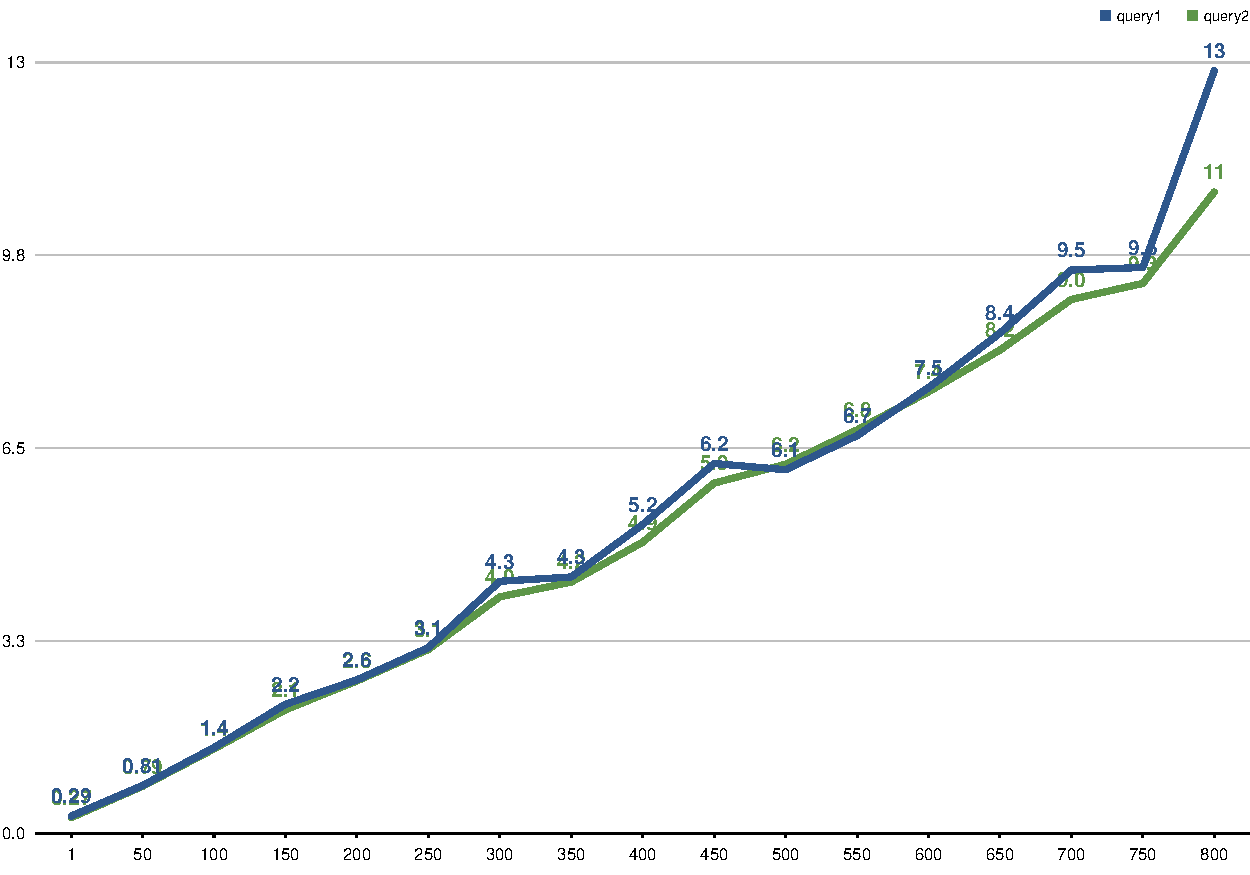
\includegraphics[width=\textwidth]{charts/execution-time-file-fdw-number_of_values}
        \caption{wersja z \texttt{file\_fdw}}
    \end{subfigure}
    \hfill
    \begin{subfigure}{.49\textwidth}
        \centering
        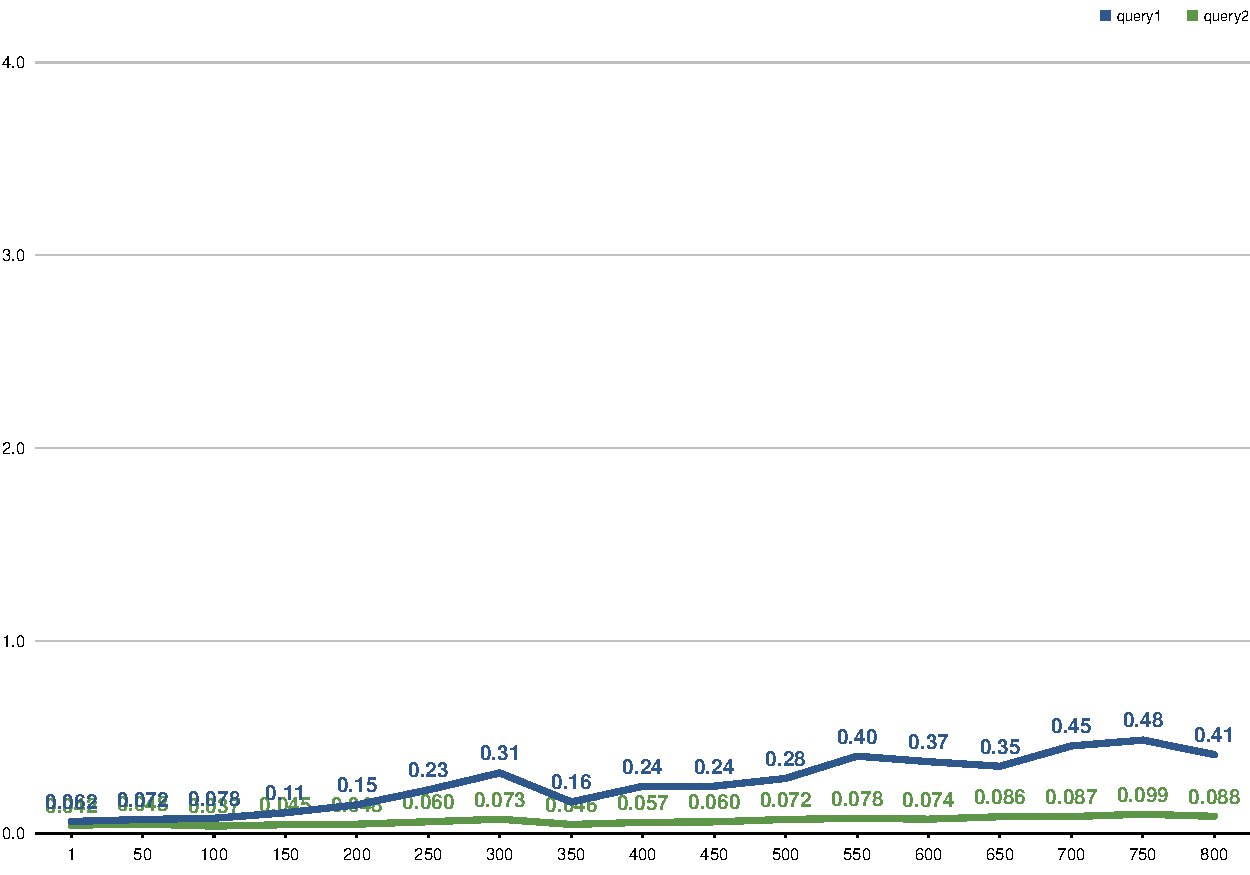
\includegraphics[width=\textwidth]{charts/execution-time-sql-one-table-number_of_values}
        \caption{wersja z jedną tabelą}
    \end{subfigure}
    \begin{subfigure}{.5\textwidth}
        \centering
        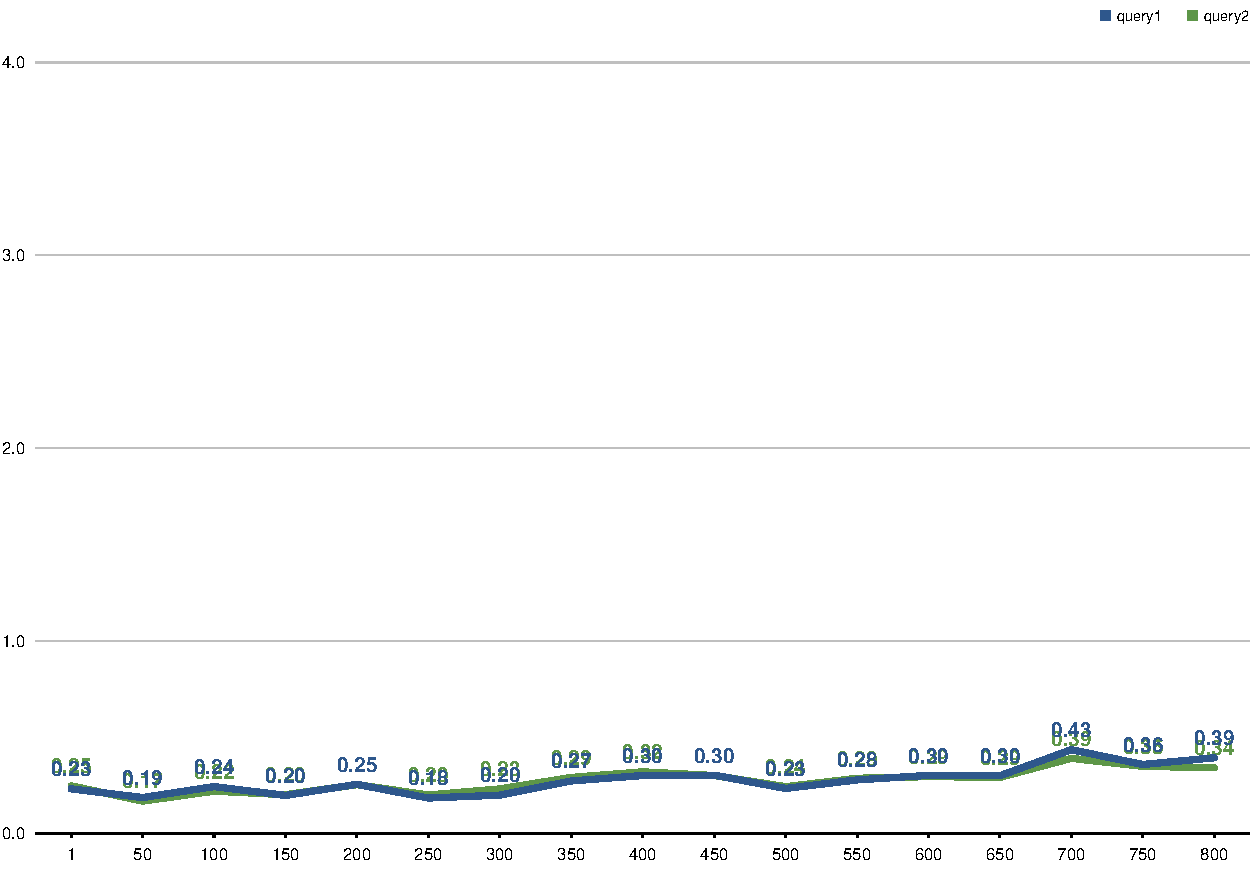
\includegraphics[width=\textwidth]{charts/execution-time-cstore-fdw-number_of_values}
        \caption{wersja z \texttt{cstore\_fdw}}
    \end{subfigure}
    \caption{Średni czas wykonania (w milisekundach) w zależności od liczby kolumn z wartościami.}
    \label{execution-time-number-of-values}
\end{figure}


\subsection{Porównanie wydajności w zależności od długości przedziałów dat w pytaniach}

Dane wykorzystane w tym teście mają 8000 dni, 10 kategorii i 10 kolumn z wartościami. Za każdym razem jest to więc 80\,000 wierszy.
Na rysunku \ref{execution-time-distance-in-days} widać, że czas wykonania wersji korzystającej z~\texttt{file\_fdw} rośnie
powoli, a pozostałych dwóch szybko. Nadal jednak jest ona najwolniejsza.
\begin{figure}[h!]
    \centering
    \begin{subfigure}{.49\textwidth}
        \centering
        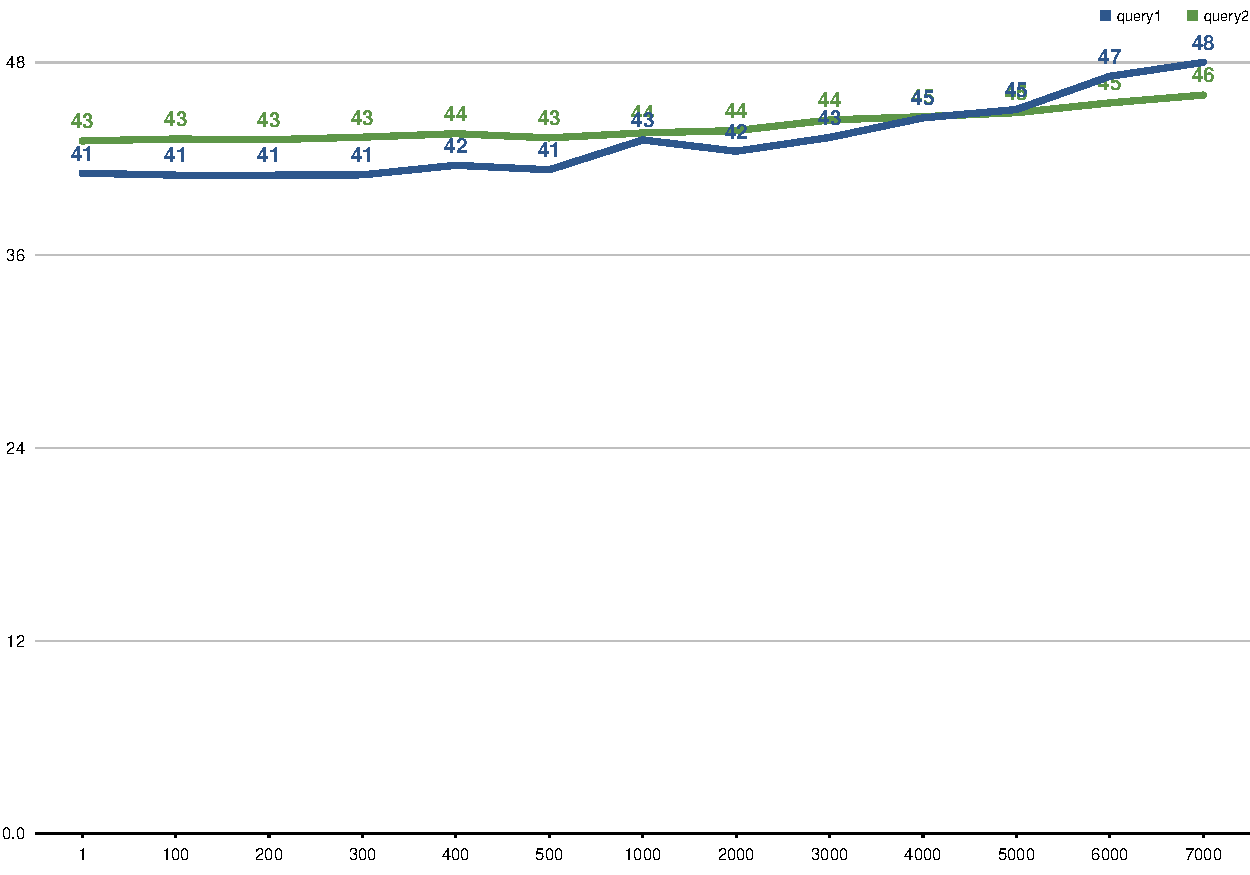
\includegraphics[width=\textwidth]{charts/execution-time-file-fdw-distance_in_days}
        \caption{wersja z \texttt{file\_fdw}}
    \end{subfigure}
    \hfill
    \begin{subfigure}{.49\textwidth}
        \centering
        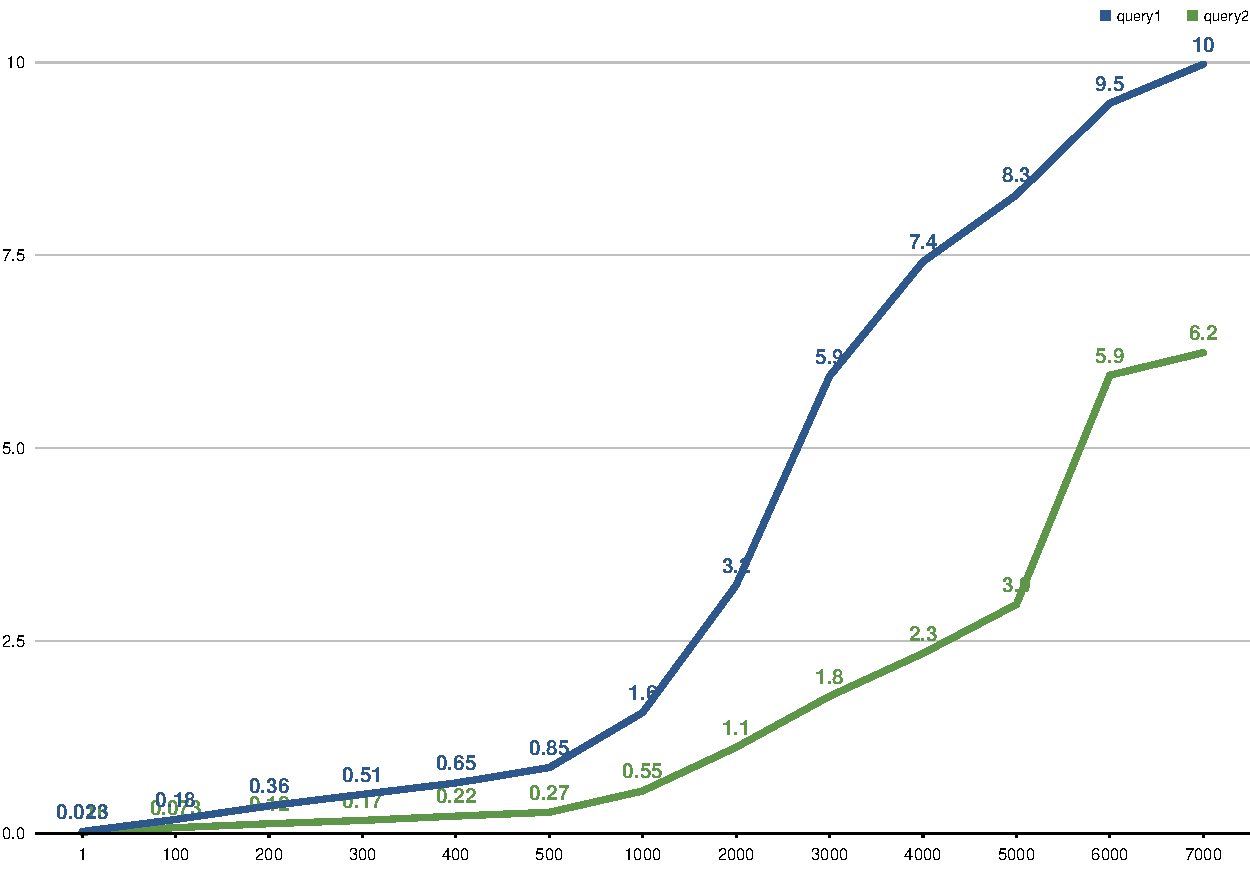
\includegraphics[width=\textwidth]{charts/execution-time-sql-one-table-distance_in_days}
        \caption{wersja z jedną tabelą}
    \end{subfigure}
    \begin{subfigure}{.5\textwidth}
        \centering
        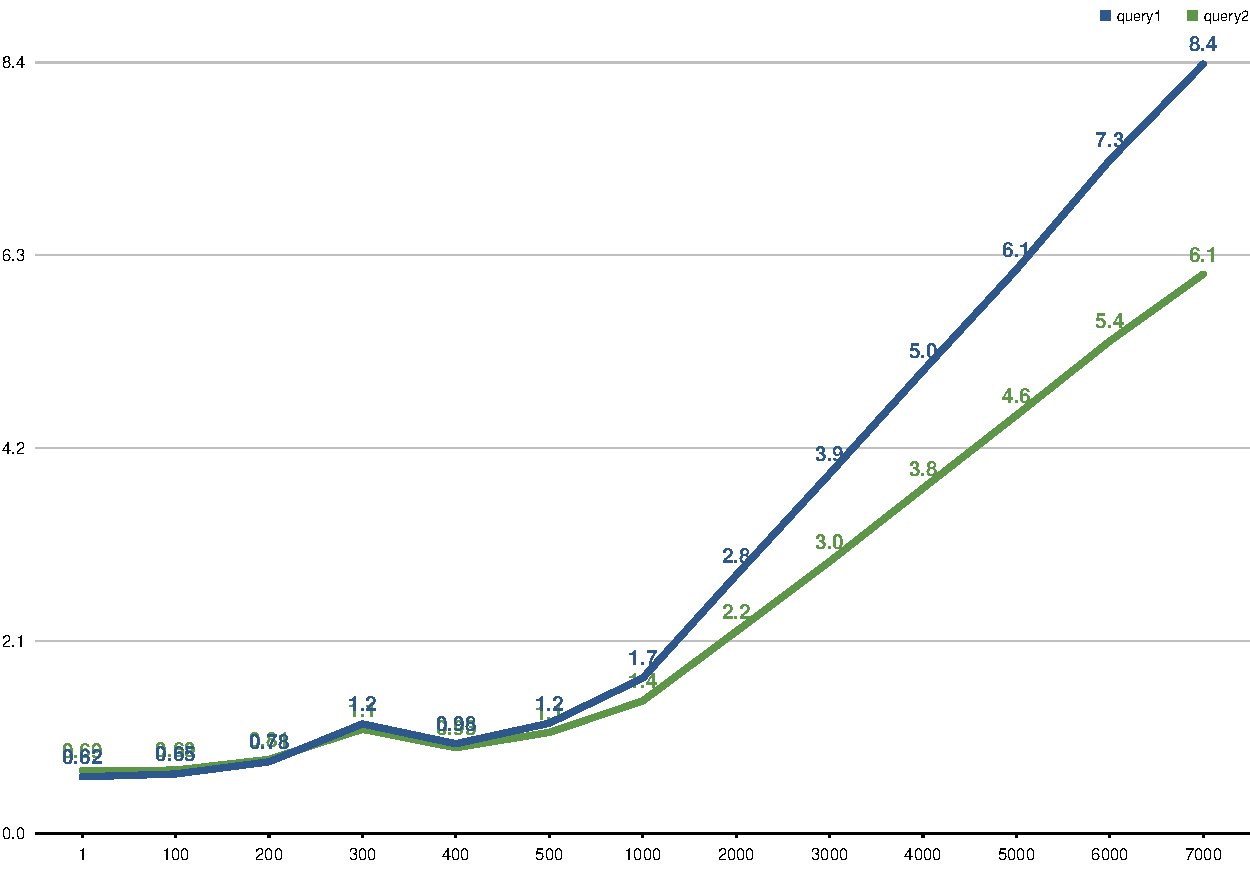
\includegraphics[width=\textwidth]{charts/execution-time-cstore-fdw-distance_in_days}
        \caption{wersja z \texttt{cstore\_fdw}}
    \end{subfigure}
    \caption{Średni czas wykonania (w milisekundach) w zależności od długości przedziałów dat.}
    \label{execution-time-distance-in-days}
\end{figure}


\subsection{Porównanie wydajności w zależności od liczby kategorii}

W tym porównaniu (wykresy na rysunku \ref{execution-time-number-of-categories}) czasy wykonania wszystkich wersji
rosną dość szybko. Ponownie wersja z jedną tabelą w postgresie i z \texttt{cstore\_fdw} są o wiele szybsze
od pierwszej. Warto zauważyć przewagę wykonania zapytania \texttt{query2} w wersji drugiej.
\begin{figure}[h!]
    \centering
    \begin{subfigure}{.49\textwidth}
        \centering
        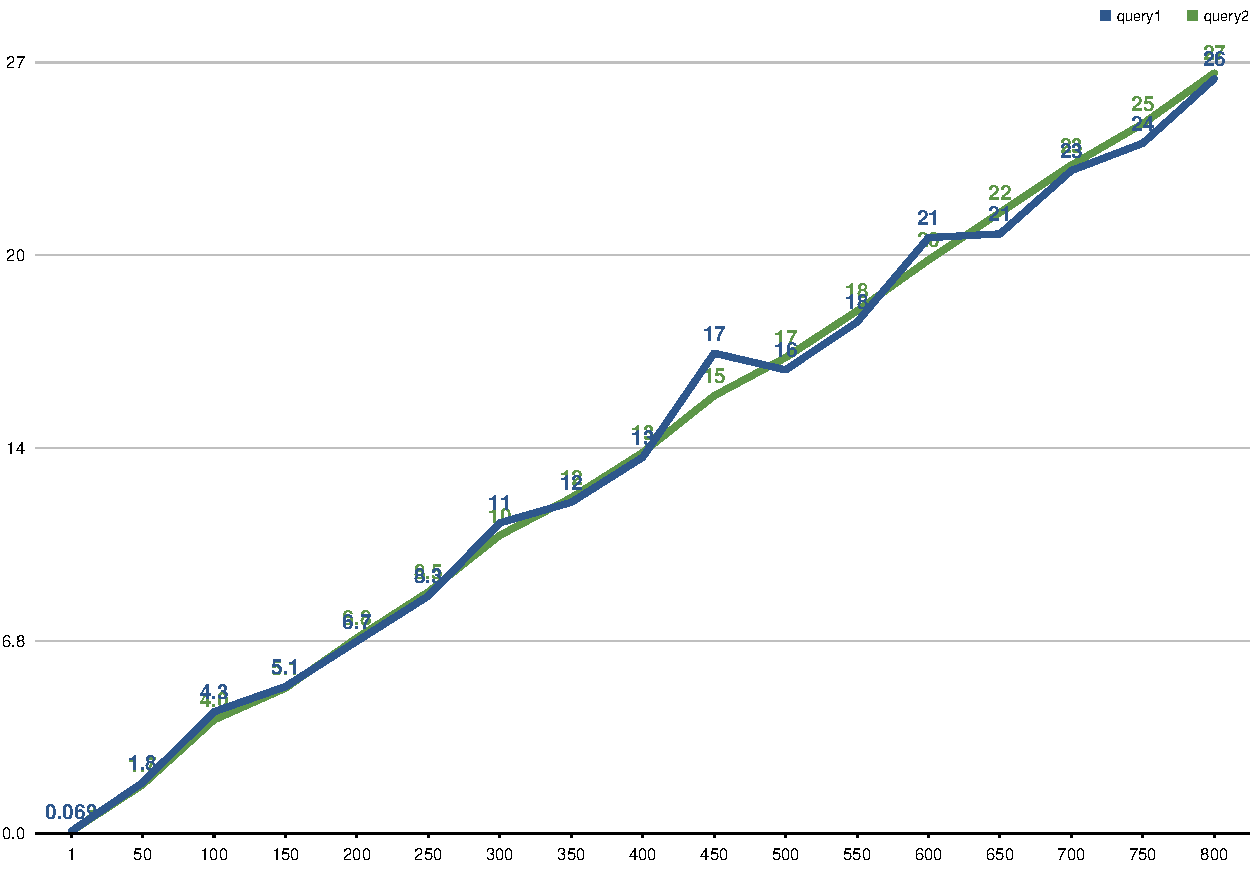
\includegraphics[width=\textwidth]{charts/execution-time-file-fdw-number_of_categories}
        \caption{wersja z \texttt{file\_fdw}}
    \end{subfigure}
    \hfill
    \begin{subfigure}{.49\textwidth}
        \centering
        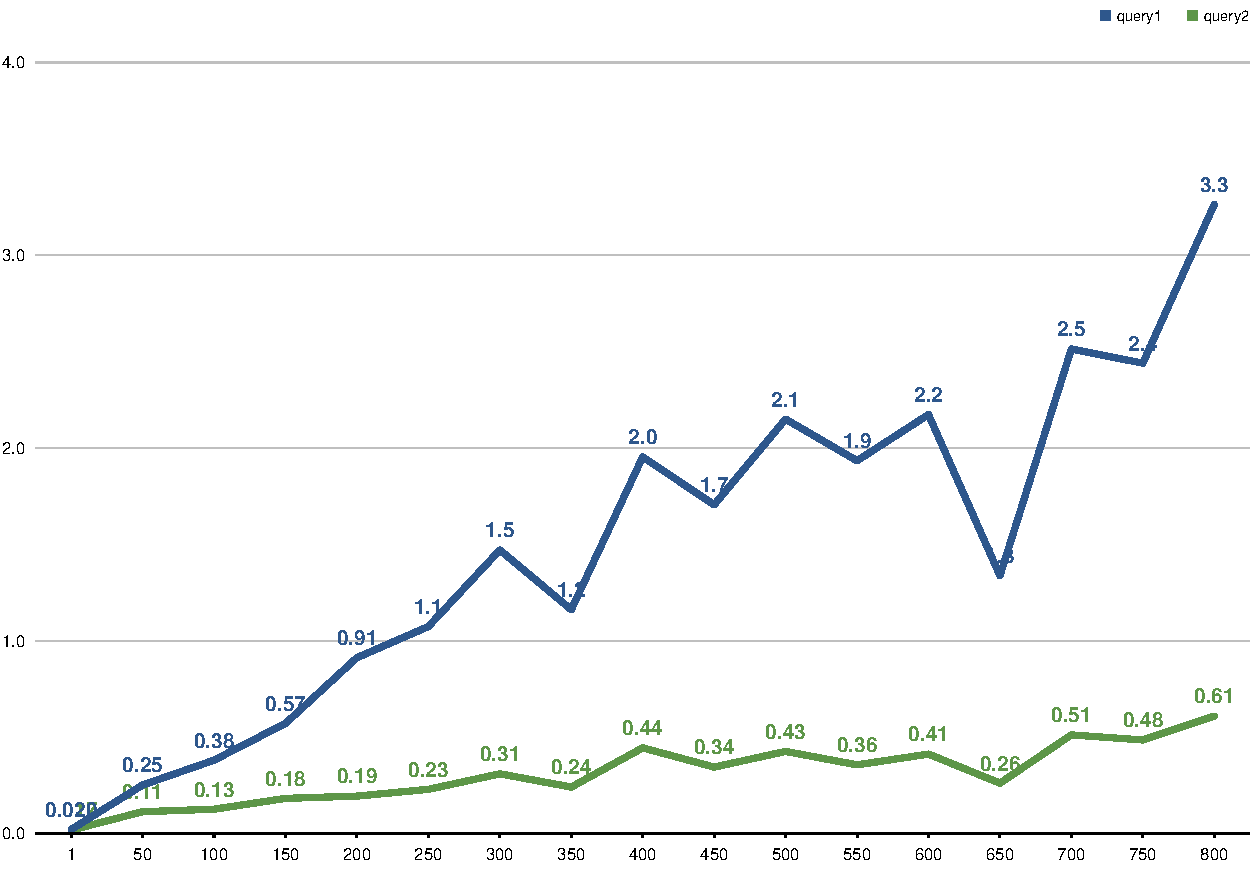
\includegraphics[width=\textwidth]{charts/execution-time-sql-one-table-number_of_categories}
        \caption{wersja z jedną tabelą}
    \end{subfigure}
    \begin{subfigure}{.5\textwidth}
        \centering
        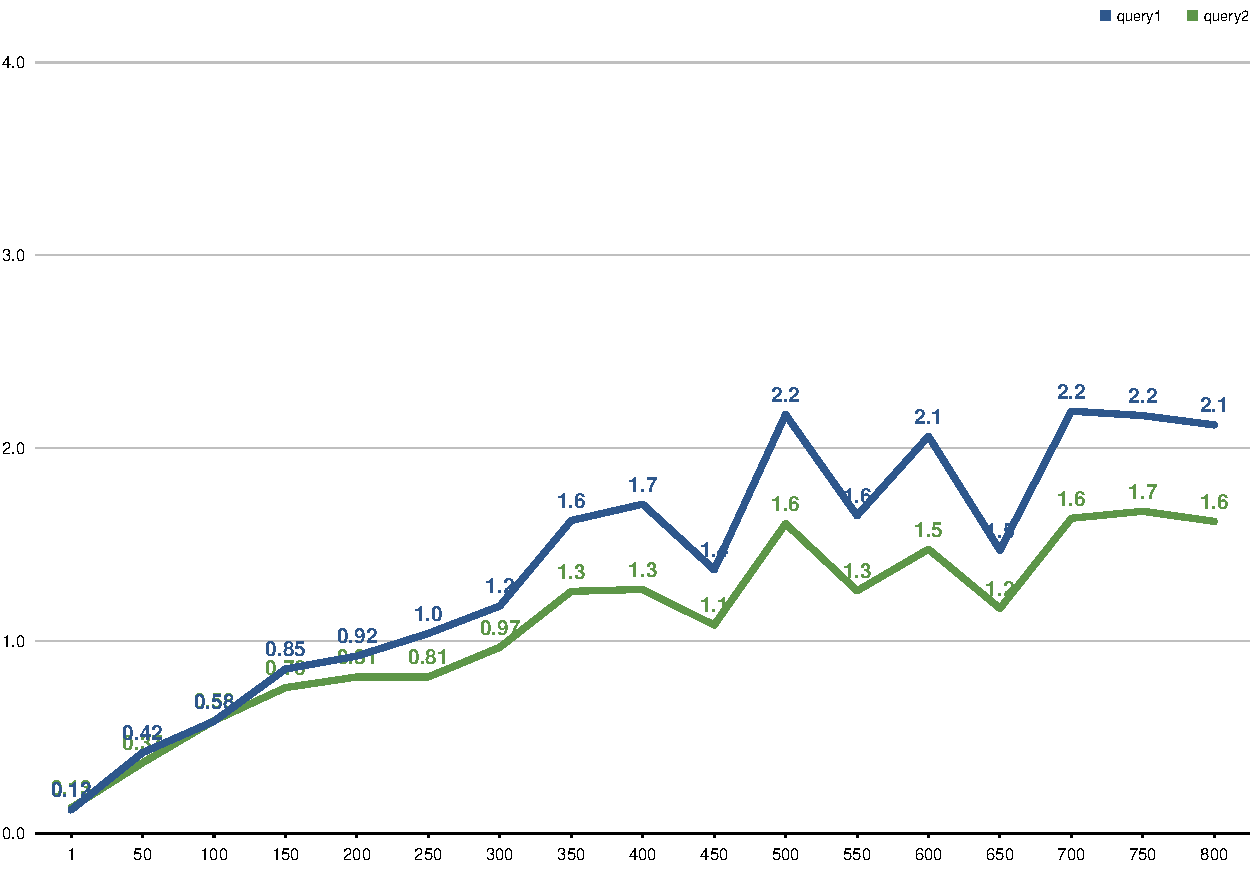
\includegraphics[width=\textwidth]{charts/execution-time-cstore-fdw-number_of_categories}
        \caption{wersja z \texttt{cstore\_fdw}}
    \end{subfigure}
    \caption{Średni czas wykonania (w milisekundach) w zależności od liczby występujących kategorii.}
    \label{execution-time-number-of-categories}
\end{figure}


\subsection{Porównanie rozmiaru plików z danymi}

Ten punkt pokazuje rozmiary plików z danymi w wersji korzystającej z jednej tabeli w postgresie
i~z~\texttt{cstore\_fdw}. Na rysunku \ref{size-of-data-file} widzimy rozmiary w zależności od liczby
kolumn z wartościami oraz w~zależności od liczby kategorii. Dla danych z testu długości przedziałów dat,
pliki mają stały rozmiar --- 6\,000 KiB (wersja z jedną tabelą) i 4\,200 KiB (\texttt{cstore\_fdw}).
\begin{figure}[h!]
    \centering
    \begin{subfigure}{.49\textwidth}
        \centering
        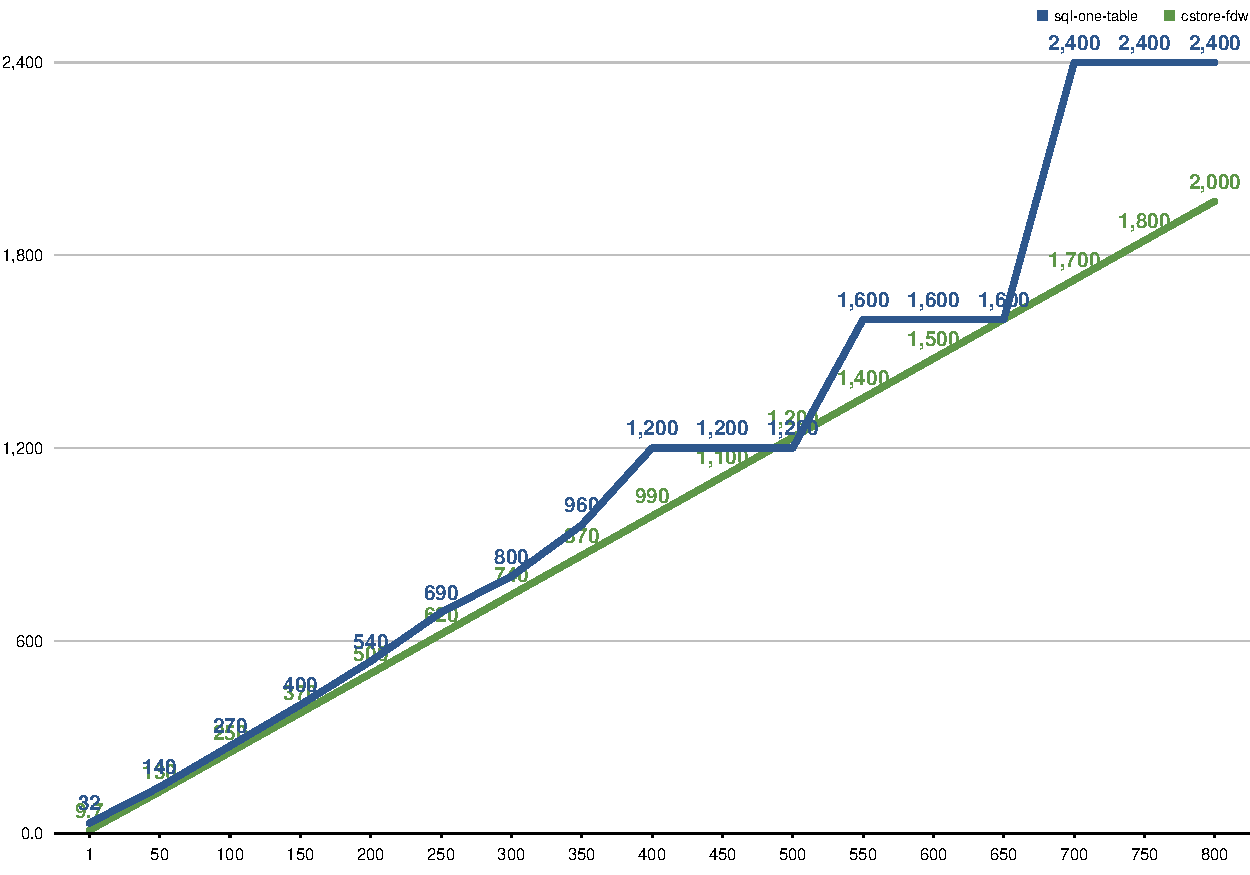
\includegraphics[width=\textwidth]{charts/size-of-data-file-number_of_values}
        \caption{w zależności od liczby kolumn z wartościami}
    \end{subfigure}
    \hfill
    \begin{subfigure}{.49\textwidth}
        \centering
        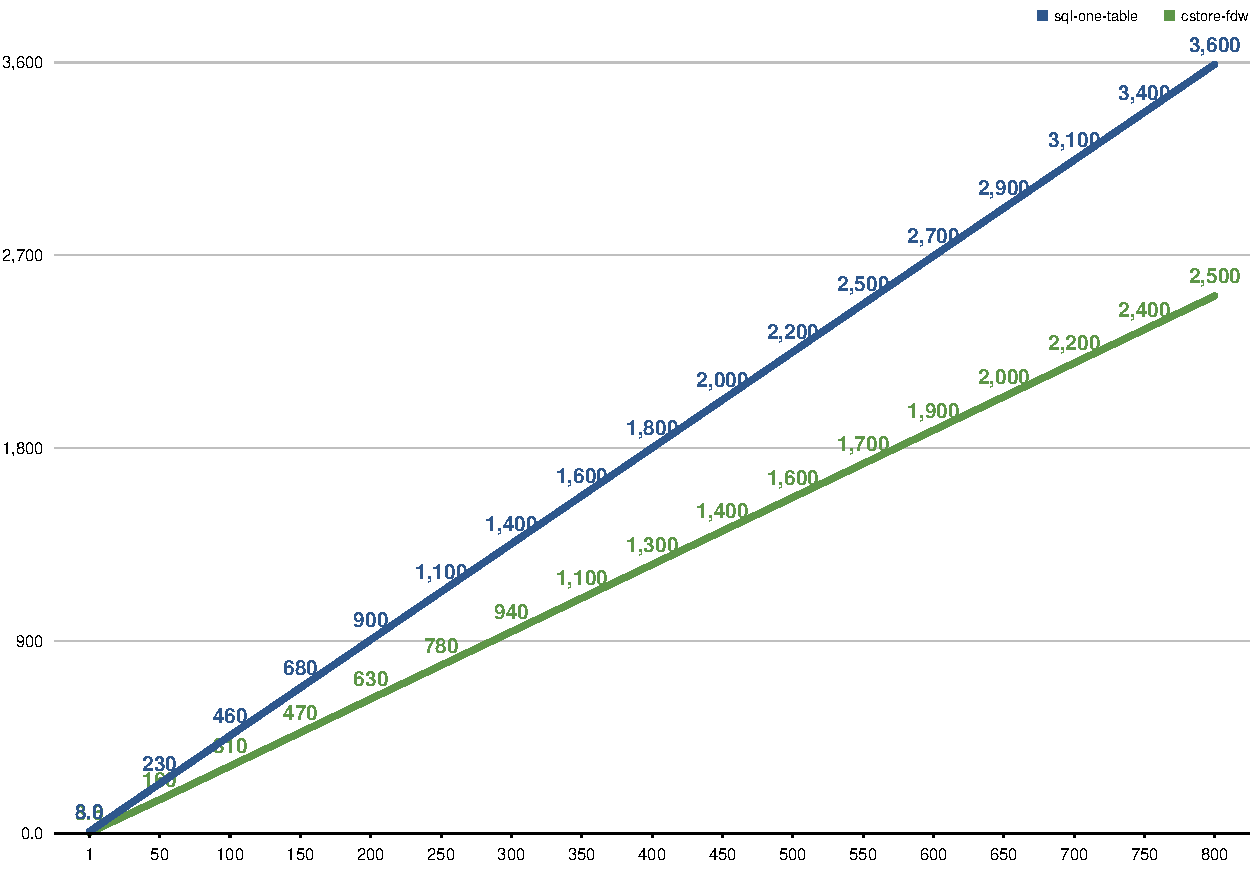
\includegraphics[width=\textwidth]{charts/size-of-data-file-number_of_categories}
        \caption{w zależności od liczby kategorii}
    \end{subfigure}
    \caption{Rozmiar plików z danymi (w kibibajtach).}
    \label{size-of-data-file}
\end{figure}


\subsection{Wersja korzystająca z jednej tabeli w postgresie, bez klucza głównego}

W tym porównaniu tworzymy tabelę bez klucza głównego, a więc również bez związanego z nim indeksu.
Rysunek \ref{execution-time-sql-one-table-no-pk} przedstawia wykresy czasu wykonania w zależności
od liczby kolumn z wartościami, od długości przedziałów dat oraz od liczby kategorii.
Na pierwszym czasy są około 1.5--2 razy gorsze od odpowiadających im w wersji z indeksem.
Na drugim, dla długich przedziałów czasy są takie same, ale dla krótkich są kolkukrotnie większe.
Na ostatnim czasy też są większe, szczególnie dla zapytania drugiego.

Być może dobrym wykorzystaniem indeksów byłoby stworzenie tabeli z czterema kolumnami --- datą,
kategorią, numerem wartości i wartością oraz indeksami na trzech pierwszych kolumnach.
\begin{figure}[h!]
    \centering
    \begin{subfigure}{.49\textwidth}
        \centering
        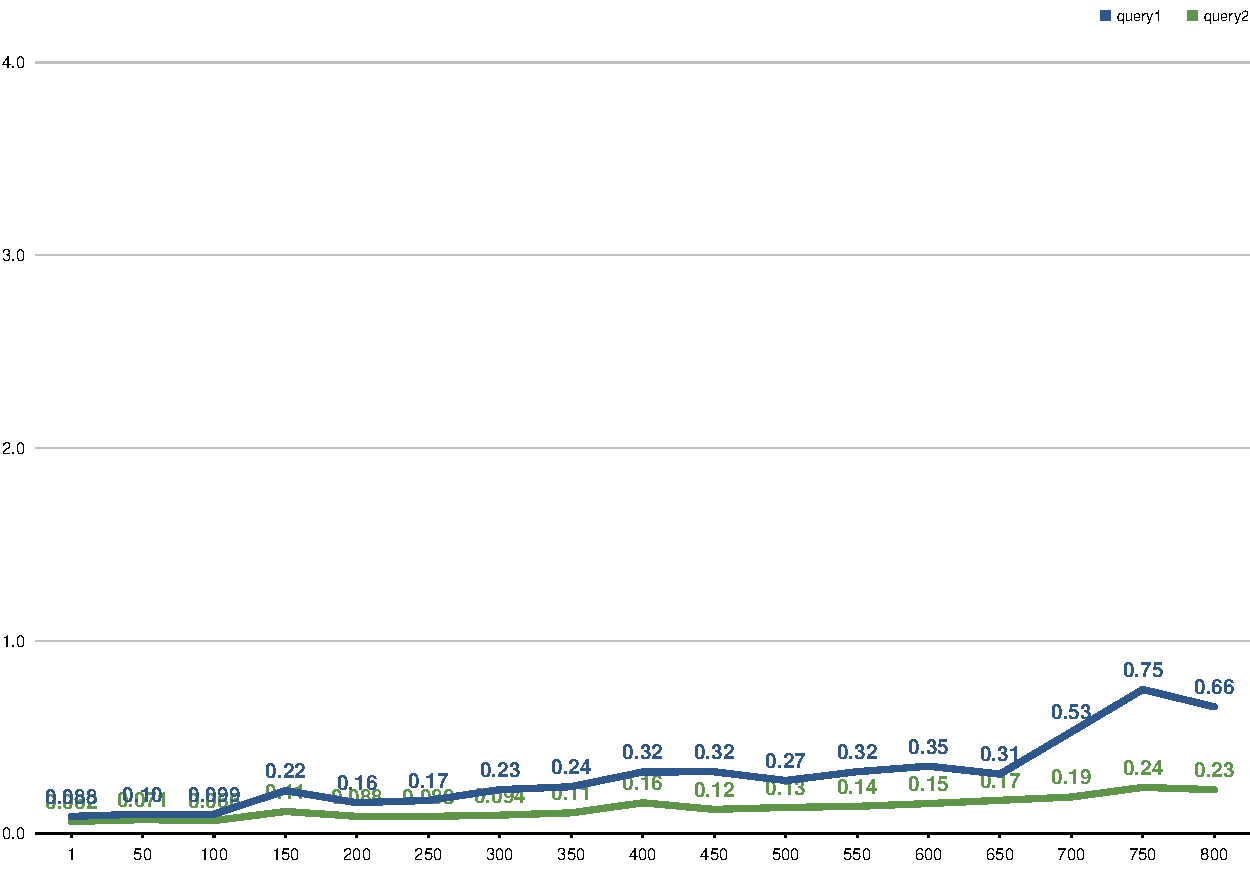
\includegraphics[width=\textwidth]{charts/execution-time-sql-one-table-no-pk-number_of_values}
        \caption{w zależności od liczby kolumn z wartościami}
    \end{subfigure}
    \hfill
    \begin{subfigure}{.49\textwidth}
        \centering
        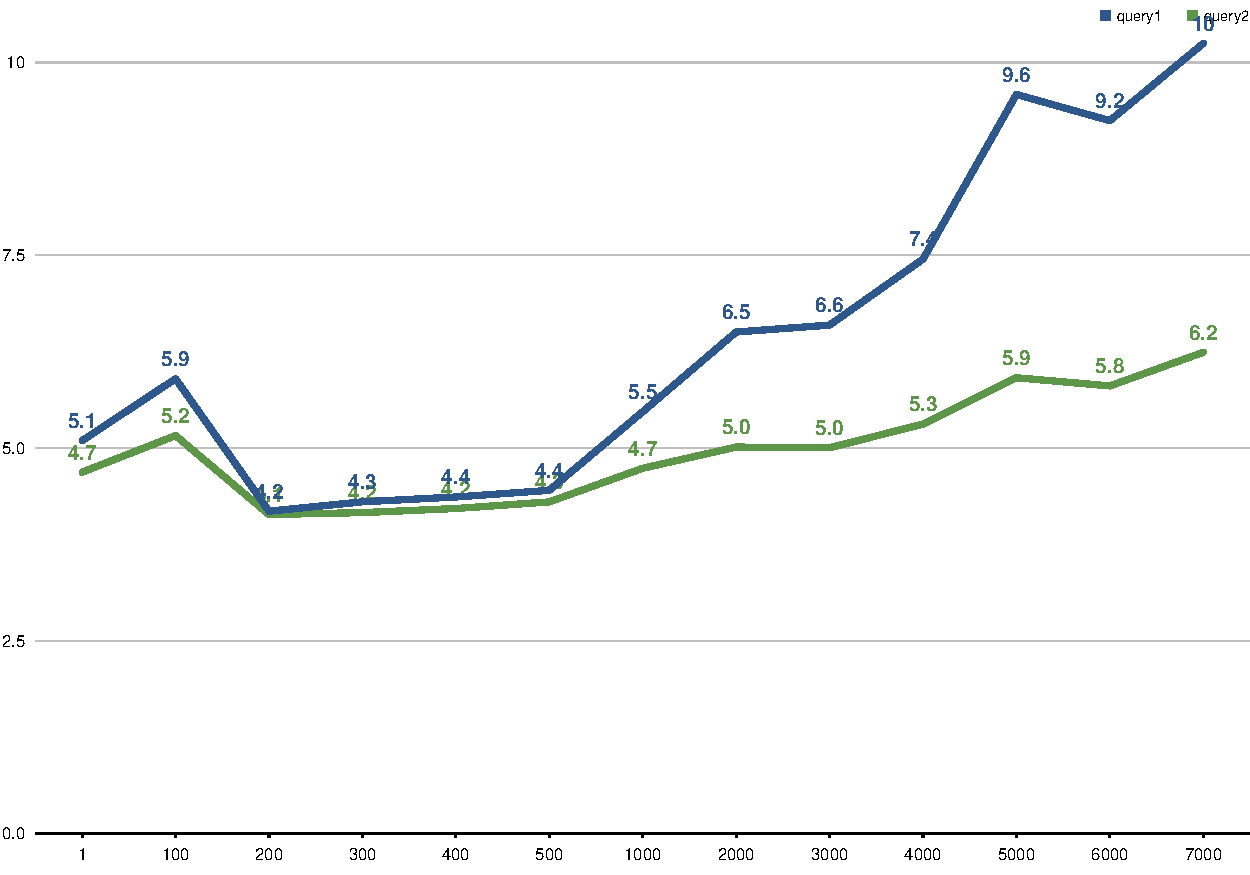
\includegraphics[width=\textwidth]{charts/execution-time-sql-one-table-no-pk-distance_in_days}
        \caption{w zależności od długości przedziałów dat}
    \end{subfigure}
    \begin{subfigure}{.5\textwidth}
        \centering
        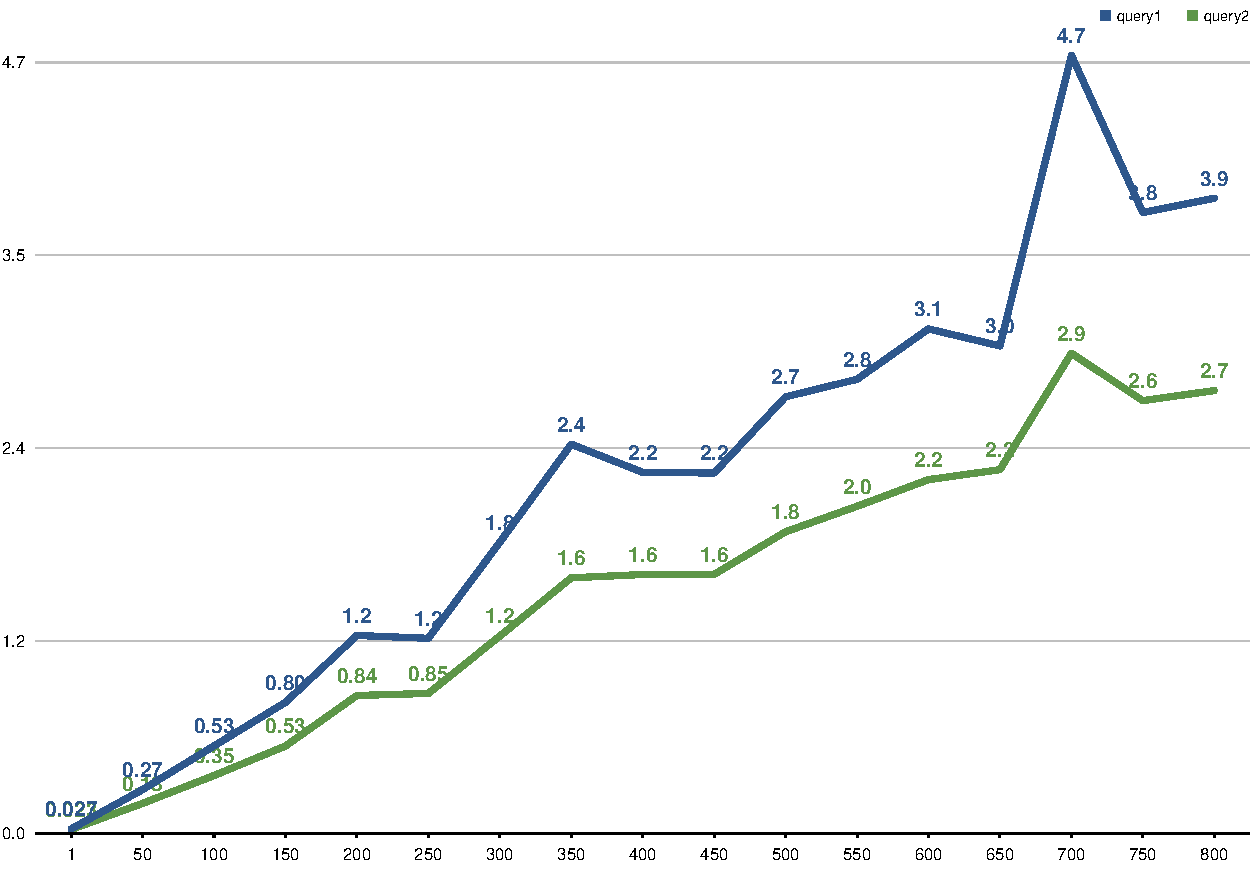
\includegraphics[width=\textwidth]{charts/execution-time-sql-one-table-no-pk-number_of_categories}
        \caption{w zależności od liczby kategorii}
    \end{subfigure}
    \caption{Średni czas wykonania (w milisekundach) dla jednej tabeli w postgresie bez klucza głównego.}
    \label{execution-time-sql-one-table-no-pk}
\end{figure}


\section{Podsumowanie}

W każdym porównaniu wersja korzystająca z \texttt{file\_fdw} wypada najsłabiej.
Pozostałe dwie wersje w~niektórych przypadkach nieznacznie różnią się na korzyść pierwszej z nich,
ale w~innych na korzyść drugiej. Całościowo określiłbym ich wyniki jako równoważne.


\end{document}
